\documentclass{BeamerTemplate}

\title{Module 8.1 - Tests d'hypothèses à un échantillon}

\graphicspath{{Images/Module 8/}}

\begin{document}
\begin{frame}[t]
  \titlepage
\end{frame}

%-------------------------------------------------------------------------------------------------------------------------------------





%%%%%%%%%%%%%%%%%%%%%%%%%%%%%%%%%%%
%%%%%%%%%%%%%%%%%%%%%%%%%%%%%%%%%%%
%%%%%%%%%%%%%%%%%%%%%%%%%%%%%%%%%%%

\section{Introduction}


\subsection*{ }

\begin{frame}[t]{Des hypothèses de recherche}
Une question de recherche est souvent liée à un paramètre d'une population d'intérêt :
\bigskip

\begin{itemize}\itemsep 5mm
%\item la proportion de ch\^omeurs dans une région est inférieure à 6\%;
\item Le taux moyen de défaillance des circuits imprimés produits par une nouvelle ligne de soudure est inférieur à 2\%.
\item La durée moyenne d’assemblage d’un composant est réduite après l’introduction d’un nouvel outil automatisé.
\item L’écart-type des vibrations mesurées en vol sur une aile équipée d’un nouvel aileron est inférieur à celui mesuré avec l’ancien design.
\end{itemize}
\end{frame}

\begin{frame}[t]{Hypothèse statistique}

\begin{Boite}{Hypothèse statistique}{Énoncé sur la loi de probabilité que suit une variable aléatoire.}
\end{Boite}

\medskip
Exemples:%, si $X_1, \ldots, X_n$ sont des v.a. i.i.d. $N(\mu, \sigma^2)$, alors des hypothèses statistiques possibles sont
\medskip

\begin{tabular}{p{5cm}p{5cm}}
Une population & Plusieurs populations\\
\begin{itemize}
\item $\mu \ne 10$
\item $\mu > 3$
\item $\sigma^2 = 4$
\end{itemize}
&
\begin{itemize}
\item $\mu_1 > \mu_2$
\item $\sigma^2_1 \ne \sigma^2_2$
\item $\mu_1=\mu_2=\mu_3=\mu_4$
\end{itemize}
\end{tabular}
\end{frame}



% \begin{frame}[t]{Test d'hypothèses}

% \small
% Dans un \alert{test d'hypothèses}, on confronte deux hypothèses.\\ %, dénotées $H_0$ et $H_1$.
% Par exemple,
% $$H_0 : \mu = 10 \qquad \mbox{ contre } \qquad  H_1 : \mu > 10.$$

% \medskip
%  \alert{$H_0$ : l'hypothèse nulle}. Considérée vraie {\it a priori}, par défaut,
%  le {\it status quo}.

% \medskip
% \uncover<2->{
%  \alert{$H_1$ : l'hypothèse alternative}.
% C'est l'hypothèse que les données permettent de démontrer.}

% \medskip
% \uncover<3->{
% On suppose que $H_0$ est vraie jusqu'à ce qu'une \underline{preuve suffisante (significative)} que $H_0$ n'est pas vraie ait été amassée. La preuve provient des données qui sont observées.}

% \end{frame}


\begin{frame}[t]{Test d'hypothèses}

\small
Dans un \alert{test d'hypothèses}, on confronte deux hypothèses.\\ %, dénotées $H_0$ et $H_1$.
Par exemple,
$$H_0 : \mu = 10 \qquad \mbox{ contre } \qquad  H_1 : \mu > 10.$$

\medskip
 \alert{$H_0$ : l'hypothèse nulle}. Hypothèse supposée vraie en l’absence de preuve suffisante du contraire.

\medskip

 \alert{$H_1$ : l'hypothèse alternative}.
Hypothèse soutenue par les données si celles-ci fournissent suffisamment d’éléments pour rejeter $H_0$. Elle incarne un changement ou un effet à détecter.

\medskip

On suppose que $H_0$ est vraie jusqu'à ce qu'une \underline{preuve suffisante (significative)} que $H_0$ n'est pas vraie ait été amassée. La preuve provient des données qui sont observées.

\end{frame}


\begin{frame}[t]{Remarques}
\begin{itemize}\itemsep4mm
\item $H_0$ et $H_1$ sont toujours mutuellement exclusives.
\item $H_1$ peut avoir une forme bilatérale ($\mu\ne 10$)\\ ou unilatérale ($\mu<10$ ou $\mu>10$)
\item C'est l'hypothèse de recherche (ce qui doit être démontré à partir de données) qui dicte le sens de $H_1$.

\end{itemize}
\end{frame}

\begin{frame}[t]{ }

\centerline{\LARGE\bf \alert{QUIZ !}}
\bigskip

Vous devez valider qu'une structure de béton a une résistance moyenne supérieure à 80 MPa. Vous prélèverez 10 carottes à analyser.
\bigskip

\begin{enumerate}\itemsep 15mm
\item Quelles sont vos hypothèses statistiques?
\item Vous obtenez une moyenne échantillonnale de $\overline x = 81,6$ MPa. Pouvez-vous conclure quelque chose? \href{https://jmiron-introtest.share.connect.posit.cloud/}{Illustration}
\end{enumerate}

\vspace{1.5cm}
\end{frame}

\begin{frame}[t]{Étapes d'un test d'hypothèses}

\begin{enumerate}
    \item On détermine les hypothèses $H_0$ et $H_1$ à confronter.
    \item On recueille un échantillon aléatoire.
    \item On décide si l'échantillon recueilli à l'étape 2 contient
    suffisamment de preuves pour rejeter $H_0$ en faveur de $H_1$ ou pas.
\end{enumerate}

\bigskip

{\bf Il nous faut donc une règle pour prendre la décision à l'étape 3.}

\end{frame}

\begin{frame}[t]{Règle de décision}

Il n'y a que deux résultats possibles à un test d'hypothèse : \alert{rejeter} $H_0$ ou
\alert{ne pas rejeter} $H_0$.
\bigskip

Une règle de décision est formulée \underline{avant} d'observer les données. Elle  prend la forme d'une \alert{région critique} qui définit pour quels échantillons $H_0$ sera rejetée.

\bigskip

Par exemple, pour
$$H_0 : \mu = 10 \qquad \mbox{ contre } \qquad  H_1 : \mu > 10,$$

on devra trouver à partir de quelle valeur $k$ on décide de rejeter $H_0$.

\bigskip

\end{frame}

\begin{frame}{Loi de $\overline X$ sous $H_0$}
    \begin{tikzpicture}[xscale=2, yscale=8]

% Paramètres
\def\moy{0}
\def\sigma{1}

% Axes
\draw[->] (-3.5,0) -- (3.5,0) node[right] {$x$};
\draw[->] (0,0) -- (0,0.45) node[above] {$f(x)$};

% Densité normale
\draw[thick, smooth, domain=-3:3, samples=200]
  plot (\x, {1/(\sigma*sqrt(2*pi)) * exp(-((\x-\moy)^2)/(2*\sigma^2))});

% Repères optionnels
\draw[dashed] (-3,0) -- (-3,0.004);
\draw[dashed] (3,0) -- (3,0.004);
\node at (0,-0.03) {$\mu=10$};

\end{tikzpicture}
\end{frame}
\begin{comment}
\begin{frame}[t]{Types d'erreur possibles}
Comme on a affaire à des variables aléatoires, même avec une excellente règle
de décision il n'est pas certain
que nous prendrons toujours la bonne décision. Nous pouvons nous tromper de deux fa\c{c}ons:
\begin{itemize}
\item<1-> \alert{\bf Erreur de première espèce (ou erreur de type I):} on rejette $H_0$ alors qu'elle est vraie.
\item<2-> \alert{\bf Erreur de deuxième espèce (ou erreur de type II):} on ne rejette pas $H_0$ alors qu'elle est fausse.
\end{itemize}
\end{frame}
\end{comment}
\begin{frame}[t]{Deux erreurs possibles à l'issue d'un test d'hypothèses}

{\small
\begin{center}
\begin{tabular}{|c||c|c|}\cline{2-3}
\multicolumn{1}{c||}{ }&\multicolumn{2}{c|}{\bf Réalité (inconnue!)}\\\hline
{\bf Décision} & $  {H_0}$   est vraie  & $ {H_0}$  est fausse \\ \hline\hline
  On rejette $ H_0 $ & \alert{Erreur de type I} & \\ \hline
  On ne rejette pas  $ H_0 $ & & \alert{Erreur de type II} \\ \hline
\end{tabular}
\end{center}


%Les règles de décision doivent limiter les chances de commettre des erreurs.


\vspace{3mm}

$\begin{array}{lcl}
\begin{array}{ll}
\alert{\alpha}&=P(\text{erreur de type I})\\
&= P(\text{rejeter }H_0 | H_0\text{\ vraie})\\
&= \textbf{\underline{seuil} du test}\\ &\\
\end{array}  & \textbf{ET} & \\ 
\begin{array}{ll}
\alert{\beta}&=P(\text{erreur de type II}) \\
&= P(\text{ne pas rejeter }H_0 | H_0\text{\ fausse})\\
&= P(\text{ne pas rejeter }H_0 | H_1\text{\ vraie})\\
\end{array}
& \Leftrightarrow &
\begin{array}{ll}
\alert{1-\beta}&=P(\text{rejeter }H_0 | H_0\text{\ fausse})\\
&= P(\text{rejeter }H_0 | H_1\text{\ vraie})\\
&= \textbf{\underline{puissance} du test}\\&\\
\end{array}
\end{array}$
}

\end{frame}

\begin{frame}{Loi de $\overline X$ sous $H_0$}
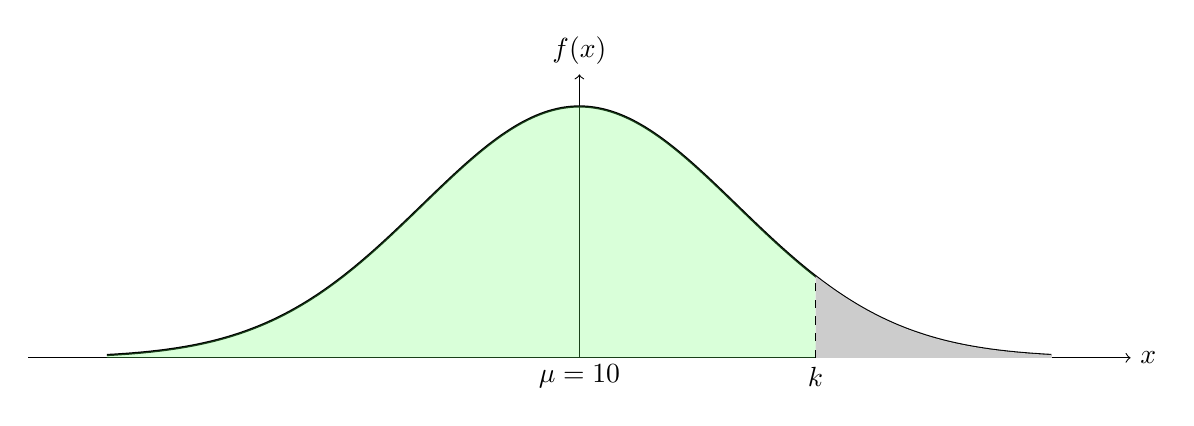
\begin{tikzpicture}[xscale=2, yscale=8]

% Paramètres
\def\moy{0}
\def\sigma{1}
\def\a{1.5} % seuil à droite

% Axes
\draw[->] (-3.5,0) -- (3.5,0) node[right] {$x$};
\draw[->] (0,0) -- (0,0.45) node[above] {$f(x)$};

% Densité normale (courbe)
\draw[thick, smooth, domain=-3:3, samples=200]
  plot (\x, {1/(\sigma*sqrt(2*pi)) * exp(-((\x-\moy)^2)/(2*\sigma^2))});

% Région ombrée à droite de a
\path[fill=gray!40, domain=\a:3, samples=200]
  plot (\x, {1/(\sigma*sqrt(2*pi)) * exp(-((\x-\moy)^2)/(2*\sigma^2))})
  -- (3,0) -- (\a,0) -- cycle;

  \path[fill=green!60, fill opacity=0.25, domain=-3:\a, samples=200]
  plot (\x, {1/(\sigma*sqrt(2*pi)) * exp(-((\x-\moy)^2)/(2*\sigma^2))})
  -- (\a,0) -- (-3,0) -- cycle;

% Trait vertical au seuil
\draw[dashed] (\a,0) --
  (\a,{1/(\sigma*sqrt(2*pi)) * exp(-((\a-\moy)^2)/(2*\sigma^2))});

\node[below] at (\a,0) {$k$};
\node at (0,-0.03) {$\mu=10$};

\end{tikzpicture}
\end{frame}


\begin{frame}[t]{Quelques remarques}
\begin{itemize}\itemsep4mm
\item {\bf L'erreur de type I  est la plus grave}, donc $\alpha$ est fixé par le chercheur à une faible valeur (souvent $\alpha=0,05$ ou $0,01$).
\item Plus $\alpha$ est petit, plus $\beta$ est grand...\\donc on fixe $\alpha$ et contrôlera souvent $\beta$ avec la taille d'échantillon.
\end{itemize}

\vspace{3cm}

On doit maintenant trouver la valeur de $k$ qui nous donne la probabilité d'erreur de type I ($\alpha$) désirée.
\end{frame}


\begin{frame}{Loi de $\overline X$ sous $H_0$}
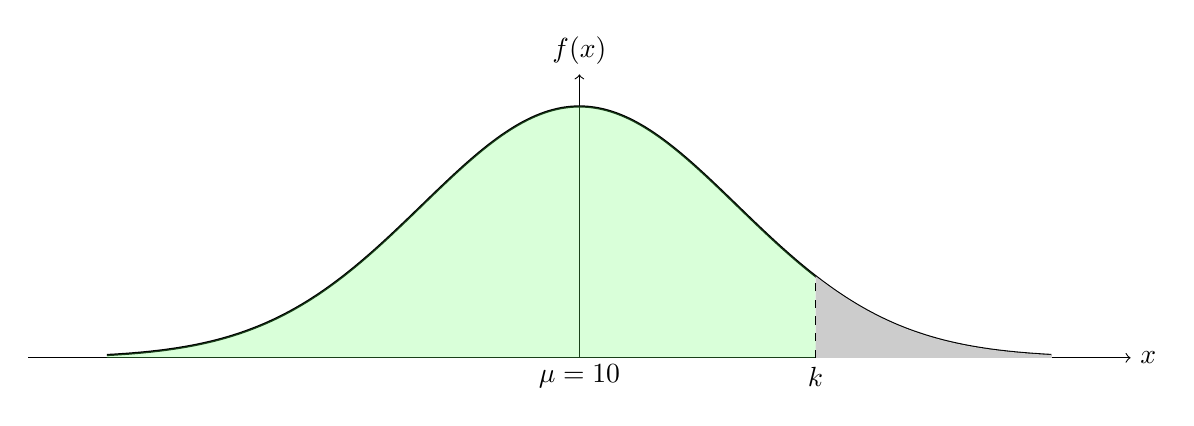
\begin{tikzpicture}[xscale=2, yscale=8]

% Paramètres
\def\moy{0}
\def\sigma{1}
\def\a{1.5} % seuil à droite

% Axes
\draw[->] (-3.5,0) -- (3.5,0) node[right] {$x$};
\draw[->] (0,0) -- (0,0.45) node[above] {$f(x)$};

% Densité normale (courbe)
\draw[thick, smooth, domain=-3:3, samples=200]
  plot (\x, {1/(\sigma*sqrt(2*pi)) * exp(-((\x-\moy)^2)/(2*\sigma^2))});

% Région ombrée à droite de a
\path[fill=gray!40, domain=\a:3, samples=200]
  plot (\x, {1/(\sigma*sqrt(2*pi)) * exp(-((\x-\moy)^2)/(2*\sigma^2))})
  -- (3,0) -- (\a,0) -- cycle;

  \path[fill=green!60, fill opacity=0.25, domain=-3:\a, samples=200]
  plot (\x, {1/(\sigma*sqrt(2*pi)) * exp(-((\x-\moy)^2)/(2*\sigma^2))})
  -- (\a,0) -- (-3,0) -- cycle;

% Trait vertical au seuil
\draw[dashed] (\a,0) --
  (\a,{1/(\sigma*sqrt(2*pi)) * exp(-((\a-\moy)^2)/(2*\sigma^2))});

\node[below] at (\a,0) {$k$};
\node at (0,-0.03) {$\mu=10$};

\end{tikzpicture}

Si nous connaissons la loi de $\overline X$ sous $H_0$, nous sommes capable d'en déduire la valeur de $k$ qui nous donne la région critique désirée.
\end{frame}


\begin{frame}[t]{Exemple 1}
    Soit $X_1,\hdots, X_{n}$ qui sont i.i.d.  $\mathcal{N}(\mu, \sigma^2)$. On désire confronter les hypothèses:

    \begin{align*}
        H_0:\mu = 10 & & H_1:\mu>10.
    \end{align*}

    À partir de quelle valeur de $\overline X$ rejettera-t-on $H_0$ pour avoir un seuil $\alpha$?
\end{frame}

\begin{frame}[t]{Exemple 1}
    Soit $X_1,\hdots, X_{n}$ qui sont i.i.d.  $\mathcal{N}(\mu, \sigma^2)$. On désire confronter les hypothèses:

    \begin{align*}
        H_0:\mu = 10 & & H_1:\mu>10.
    \end{align*}

    Si en réalité $\mu=12$, quelle est la puissance du test?
\end{frame}


    

\begin{frame}{Graphiquement}
\begin{center}
    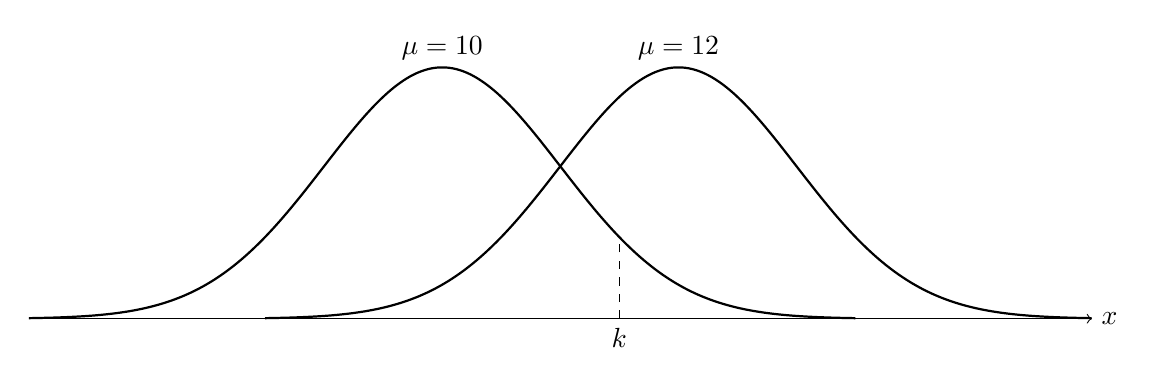
\begin{tikzpicture}[xscale=1.5, yscale=8]

% Paramètres
\def\moy{10}
\def\sigma{1}
\def\a{11.5} % seuil à droite

\def\moyy{12}
% Axes
\draw[->] (6.5,0) -- (15.5,0) node[right] {$x$};


% Densité normale (courbe)
\draw[thick, smooth, domain=6.5:13.5, samples=200]
  plot (\x, {1/(\sigma*sqrt(2*pi)) * exp(-((\x-\moy)^2)/(2*\sigma^2))});

% Densité normale (courbe)
\draw[thick, smooth, domain=8.5:15.5, samples=200]
  plot (\x, {1/(\sigma*sqrt(2*pi)) * exp(-((\x-\moyy)^2)/(2*\sigma^2))});

% Trait vertical au seuil
\draw[dashed] (\a,0) --
  (\a,{1/(\sigma*sqrt(2*pi)) * exp(-((\a-\moy)^2)/(2*\sigma^2))});


\node[below] at (\a,0) {$k$};
\node at (\moy,{1/(\sigma*sqrt(2*pi)) * exp(-((\moy-\moy)^2)/(2*\sigma^2))+0.03}) {$\mu=10$};
\node at (\moyy,{1/(\sigma*sqrt(2*pi)) * exp(-((\moyy-\moyy)^2)/(2*\sigma^2))+0.03}) {$\mu=12$};
\end{tikzpicture}
\end{center}

\end{frame}

\begin{comment}
    

\begin{frame}[t]{Exemple 1}

{\small
Une usine affirme qu'elle ne pollue pas le lac avoisinant et que la concentration moyenne de mercure dans le sol au fond du lac ne dépasse pas 0,1 ppm. \\Un biologiste souhaite démontrer le contraire.
\vspace{2mm}

Il prévoit tirer 10 prélèvements du sol au fond du lac et en mesurer la concentration de mercure. Il suppose que les concentrations sont i.i.d. $N(\mu,\;0,02^2)$. Les hypothèses sont}

\bigskip
%$H_0:~\mu=0.10$ et $H_1:~\mu>0.10$.
$H_0:$\\[4mm] $H_1:$

\end{frame}

\begin{frame}[t]{Exemple 1 (suite)}

Le biologiste hésite entre deux règles de décision.

\begin{itemize}
\item \alert{\textbf{Règle 1}}: Rejeter $H_0$ si la concentration moyenne des 10 prélèvements   est supérieure à 0,11.
\item \alert{\textbf{Règle 2}}: Rejeter $H_0$ si la concentration moyenne des 10 prélèvements   est supérieure à 0,12.
    \end{itemize}

\vspace{5mm}

\uncover<2-> { $\rightarrow$ Comment se comparent les seuils $\alpha_1$ et $\alpha_2$ associés à ces deux règles ?}

%\vspace{10mm}
%\uncover<2->{  $\rightarrow$ Si la vraie concentration moyenne est $\mu = 0,12$, laquelle des deux règles %mène à la plus grande proba\-bilité d'erreur de type II? À la plus grande puissance?}
\end{frame}

\begin{frame}[t]{Exemple 1 (suite)}

Comment se comparent les seuils associés à ces deux règles ?
\smallskip

$\alpha = P(\text{rejeter }H_0 | H_0\text{\ vraie})$

\medskip
Sous la Règle 1, on rejette $H_0$ quand $\overline{x}>0,11$. Pour calculer la probabilité
demandée, nous avons besoin de la \alert{loi échantillonnale de $\overline{X}$ quand
$H_0$ est VRAIE}, ce qui correspond à $\mu=0,1$ dans cet exemple.

\medskip

Du module 6, nous savons que cette loi est la loi 

\medskip
\uncover<2-> {Pour le seuil de la Règle 2, on remplace tout simplement 0,11 par 0,12 dans le calcul.}

\end{frame}

\begin{frame}[t]{Exemple 1 (suite)}

Le biologiste hésite entre deux règles de décision.

\begin{itemize}
\item \alert{\textbf{Règle 1}}: Rejeter $H_0$ si la concentration moyenne des 10 prélèvements   est supérieure à 0,11.
\item \alert{\textbf{Règle 2}}: Rejeter $H_0$ si la concentration moyenne des 10 prélèvements   est supérieure à 0,12.
    \end{itemize}

\vspace{5mm}

%\uncover<2->  $\rightarrow$ Comment se comparent les seuils associés à ces deux règles ?

\vspace{10mm}
\uncover<1->{  $\rightarrow$ Si la vraie concentration moyenne est $\mu = 0,12$, laquelle des deux règles mène à la plus petite proba\-bilité d'erreur de type II $\Leftrightarrow$ à la plus grande puissance?}
\end{frame}

\begin{frame}[t]{Exemple 1 (suite)}

Si la vraie concentration moyenne est $\mu = 0,12$, laquelle des deux règles mène à la plus petite proba\-bilité d'erreur de type II $\Leftrightarrow$ à la plus grande puissance $(1-\beta)$?
\smallskip

$1-\beta = P(\text{rejeter }H_0 | H_0\text{\ fausse})$

\medskip
Sous la Règle 1, on rejette $H_0$ quand $\overline{x}>0,11$. Pour calculer la probabilité
demandée, nous avons besoin de la \alert{loi échantillonnale de $\overline{X}$ quand
$H_0$ est FAUSSE}, ce qui correspond à $\mu=0,12$ dans cet exemple.

\medskip

Du module 6, nous savons que cette loi est la loi 

\medskip
\uncover<2-> {Pour la puissance de la Règle 2, on remplace tout simplement 0,11 par 0,12 dans le calcul.}

\end{frame}


\begin{frame}[t]{Exemple 1: Règle 1, rejet de $H_0$ si $\overline x > 0,11$}
\begin{center}
    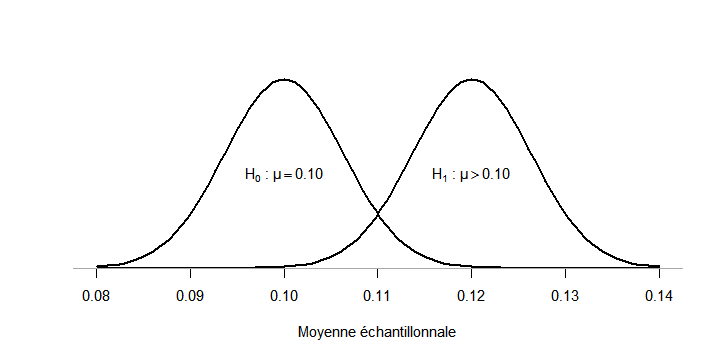
\includegraphics[scale = 0.6]{H0-xbarre.png}
\end{center}

\end{frame}


\begin{frame}[t]{Exemple  1 : Règle 2, rejet de $H_0$ si $\overline x > 0,12$}
\begin{center}
    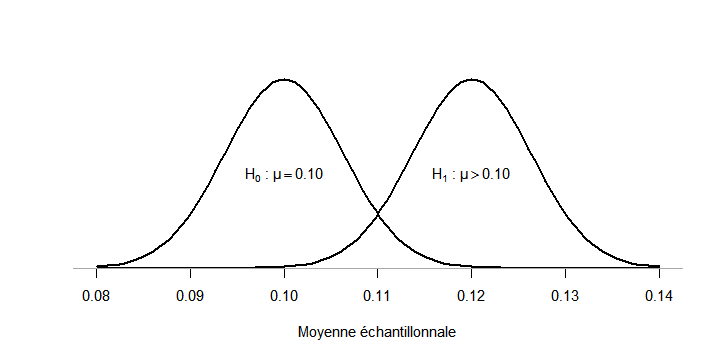
\includegraphics[scale = 0.6]{H0-xbarre.png}
\end{center}
\end{frame}

\begin{frame}[t]{Exemple  1 : Calculs complets}

Vous pourrez vérifier en exercice les valeurs des probabilités d'erreur suivantes :

\begin{center}
{\renewcommand{\arraystretch}{1.5}
\begin{tabular}{|c||c|c|}\cline{2-3}
\multicolumn{1}{c||}{ }&\multicolumn{2}{c|}{\bf Règle de décision}\\\hline
{\bf Probabilité} & Rejeter $H_0$ si $\overline x >0,11$  & Rejeter $H_0$ si $\overline x >0,12$ \\ \hline\hline
$\alpha$   & 0,057 & 0,0008\\ \hline
 $\beta$ (pour $\mu=0,12$)   & 0,057 & 0,5 \\ \hline
 $1-\beta$ (pour $\mu=0,12$)& 0,943 & 0,5 \\ \hline
\end{tabular}
}
\end{center}
{\ }
\end{frame}
\end{comment}
\section{Seuil observé / valeur-p}


\begin{frame}[t]{Le seuil observé d'un test  (valeur-p ou {\it p-value})}


%Une quantité très utilisée dans le contexte de tests d'hypothèses est le \alert{seuil observé du test}, parfois aussi appelé \alert{valeur P},  ou \alert{p-value}.
\begin{Boite}{Seuil observé, ou valeur-p}
{\small Le seuil observé d'un test (aussi appelé {\it valeur-p} ou {\it p-value}),  noté $\alpha^*$,  est la \alert{plus petite valeur de $\alpha$} pour laquelle cet échantillon nous permettrait de rejeter  $H_0$.

 \vspace{3mm}

 $\alpha^*$ peut être vu comme la \alert{probabilité d'observer un autre échantillon  ``au moins aussi extrême'' \alert{si $H_0$ est {\bf vraie}}.}}
\end{Boite}



\uncover<2->{
\begin{center}
\framebox{On rejette $H_0$ au seuil $\alpha\quad\Leftrightarrow\quad\alpha^*\le\alpha$.}



\vspace{1cm}

\href{https://jmiron-valeurp.share.connect.posit.cloud/}{Illustration}
\end{center}

}
\end{frame}



% \begin{frame}[t]{Le seuil observé d'un test (valeur-p ou {\it p-value}) VERSION 2}


% \begin{Boite}{Seuil observé / valeur-p}
% {\small Le seuil observé (ou la valeur-p) d'un test est la \alert{probabilité d'obtenir une statistique au moins aussi <<éloignée>> de $H_0$, si $H_0$ est vraie}.

%  \vspace{3mm}

%  Il s'agit de la plus petite valeur de $\alpha$ pour laquelle $H_0$ serait rejetée.
 
%  \vspace{3mm} 
%  Nous notons le seuil observé $\alpha^*$.
%  }
% \end{Boite}



% \uncover<2->{
% \begin{center}
% \framebox{On rejette $H_0$ au seuil $\alpha\quad\Leftrightarrow\quad\alpha^*\le\alpha$.}



% \vspace{1cm}

% \href{https://jmiron-valeurp.share.connect.posit.cloud/}{Illustration}
% \end{center}

% }
% \end{frame}


\begin{frame}[t]{Interprétation du seuil observé}

% La popularité du seuil observé en pratique découle du fait qu'il
 $\alpha^*$ peut s'interpréter comme %\alert{une mesure du niveau de preuve (évidence) recueillie contre $H_0$},
 \alert{une mesure de la compatibilité entre $H_0$ et les observations}, c'est la {\bf significativité statistique} du test.

\vspace{3mm}
\uncover<2->{Plus le seuil observé est \alert{faible, moins} notre échantillon semble plausible sous $H_0$.}


\vspace{3mm}
\uncover<3->{ATTENTION ! Bien qu'on rejette $H_0$ quand $\alpha^*$ est petit, sa valeur \alert{n'est {\bf PAS} la
probabilité que $H_0$ soit vraie !}}

\end{frame}

\begin{frame}[t]{Exemple 2 : Un exemple pour clarifier les choses}

{\small
On dispose d’un sac contenant \textbf{19 dés équilibrés} et \textbf{1 dé pipé} 
(ce dernier donne un «~6~» avec une probabilité de $80\%$). 
Un dé est tiré au hasard dans le sac, mais \textit{on ne sait pas lequel}. 

On lance ensuite le dé \textbf{cinq fois} de manière indépendante, et on observe 
\textbf{quatre résultats «~6~»}. 
On souhaite confronter les deux hypothèses suivantes :

\begin{align*}
    H_0 &: \text{ le dé lancé est équilibré}\\
    H_1 &: \text{ le dé lancé est pipé}
\end{align*}

Si $x$ désigne le nombre de «~6~» obtenus en cinq lancers indépendants, 
on peut définir une \textbf{région critique} de la forme $x \ge m$ où $m$ est choisi de manière à obtenir le \textbf{niveau de signification} souhaité.

\medskip
\uncover<2->{
{\bf Exercice : } Calculez $\alpha^*$. Comparez-le à la probabilité que $H_0$ soit vraie (que vous pouvez exceptionnellement
calculer ici, grâce au théorème de Bayes).}
}

\href{https://jmiron-exempledes.share.connect.posit.cloud/}{En simulation}
\end{frame}

\begin{frame}{4 cas étudiés}

La règle de rejet de $H_0$  doit être basée sur la distribution échantillonnale de notre estimateur ($\overline X$ ou $S^2$). Nous considérerons 4 situations pour les tests d'hypothèses à un échantillon (les mêmes que pour les IC):
\vspace{0.3cm}
\small

\begin{tabular}{|c|c|l|}
  \hline
  Cas&Hyp. nulle  & Situation \\\hline
&&\\[-0.3cm]
1&   & $X_1, ..., X_n\;\sim\;N(\mu, \, \sigma^2)$ avec $\sigma^2$ connue \\
&&\\
2& $H_0:\mu=\mu_0$ & $X_1, ..., X_n\;\sim\;N(\mu, \, \sigma^2)$ avec $\sigma^2$ inconnue  \\
&&\\
3&   & $X_1, ..., X_n\;\sim\;$ loi inconnue, mais $n$ est grand  \\[0.2cm]\hline
&&\\[-0.3cm]
4& $H_0:\sigma^2=\sigma^2_0$& $X_1, ..., X_n\;\sim\;N(\mu, \, \sigma^2)$ \\[0.2cm]\hline
\end{tabular}
\normalsize
\vspace{0.7cm}

\end{frame}

%%%%%%%%%%%%%%%%%%%%%%%%%%%%%%%%%%%%%%%%%%%%%%%%%%%%%%%%%%%%%%%%%%%%%%%%%%%%%%%%%%%%%
\section[1)Test sur $\mu$ ($\sigma^2$ connue)]{Cas 1: Tests d'hypothèses sur la moyenne d'une distribution normale de variance connue}

\begin{frame}[t]{Cas 1: Test sur $\mu$, loi normale, $\sigma^2$  connue}

{\color{blue}{Supposons un échantillon aléatoire  $X_1,\ldots,X_n$ issu d'une population $N(\mu, \sigma^2)$ o\`u $\mu$ est inconnue mais $\sigma^2$ est connue.}}

\bigskip
{\bf Objectif:}
Tester si l'échantillon contient suffisamment de "preuves" pour rejeter $H_0:~\mu=\mu_0$, o\`u $\mu_0$ est une valeur donnée.

\bigskip
Trois hypothèses alternatives possibles:

$H_1 : \mu \ne \mu_0$ (bilatérale) \\
$H_1 : \mu < \mu_0$ (unilatérale à gauche) \\
$H_1 : \mu > \mu_0$ (unilatérale à droite) \\
\end{frame}



\subsection{Hypothèse alternative bilatérale: $H_1 : \mu \ne \mu_0$}

\begin{frame}[t]{Hypothèse alternative unilatérale à droite}

\small
Tester $H_0 : \mu = \mu_0 \quad\mbox{ contre }\quad \alert{H_1 : \mu > \mu_0}.$

\bigskip

%On calcule $\overline{x}$ à partir de  l'échantillon.
On se doute que \alert{si $\overline{x}$ est trop élevé par rapport à $\mu_0$}, c'est que $H_0$  est probablement fausse.

\bigskip

Pour déterminer à partir de quelles valeurs $\overline x$ "est trop élevée", on
fixe le seuil $\alpha$ à une petite valeur, comme $0,05$ ou $0,01$.
\medskip

Comme nous savons comment calculer des probabilités avec la loi normale, il est possible d'utiliser la standardisation de travailler avec $Z$.

\medskip



\end{frame}


\begin{frame}[t]{Hypothèse alternative unilatérale à droite}
Autrement dit, on rejette $H_0$ au seuil $\alpha$ quand

$$
Z_0=\frac{\overline{X}-\mu_0}{\sigma/\sqrt{n}}>z_{\alpha}.
$$

\begin{minipage}{0.48\textwidth}
\centering
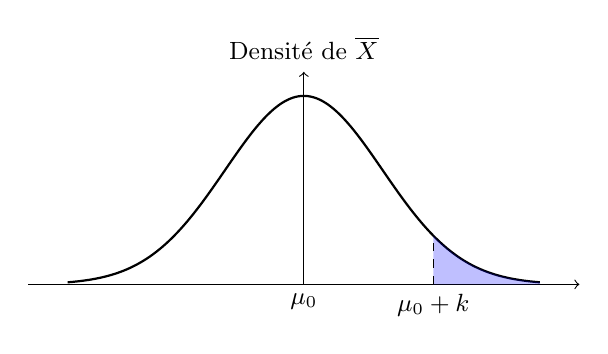
\begin{tikzpicture}[xscale=1, yscale=6]

\def\moy{0}
\def\sigma{1}
\def\a{1.645}

\draw[->] (-3.5,0) -- (3.5,0);
\draw[->] (0,0) -- (0,0.45);

\draw[thick, smooth, domain=-3:3, samples=200]
  plot (\x, {1/(\sigma*sqrt(2*pi)) * exp(-((\x-\moy)^2)/(2*\sigma^2))});

\path[fill=blue, fill opacity=0.25]
  plot[domain=\a:3, samples=200]
    (\x, {1/(\sigma*sqrt(2*pi)) * exp(-((\x-\moy)^2)/(2*\sigma^2))})
  -- (3,0) -- (\a,0) -- cycle;

\draw[dashed] (\a,0) --
  (\a,{1/(\sigma*sqrt(2*pi)) * exp(-((\a-\moy)^2)/(2*\sigma^2))});

\node[below] at (\a,0) {\small $\mu_0+k$};

\node at (0,0.5) {\small Densité de $\overline X$};
\node[below] at (0,0) {\small $\mu_0$};

\end{tikzpicture}
\end{minipage}
\hfill
\begin{minipage}{0.48\textwidth}
\centering
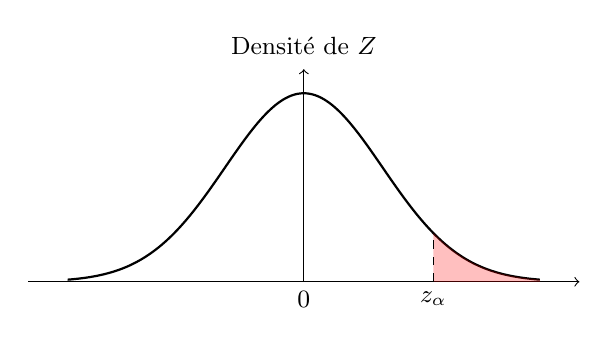
\begin{tikzpicture}[xscale=1, yscale=6]

\def\mu{0}
\def\sigma{1}
\def\a{1.645}

\draw[->] (-3.5,0) -- (3.5,0);
\draw[->] (0,0) -- (0,0.45);

\draw[thick, smooth, domain=-3:3, samples=200]
  plot (\x, {1/(\sigma*sqrt(2*pi)) * exp(-((\x-\mu)^2)/(2*\sigma^2))});

\path[fill=red, fill opacity=0.25]
  plot[domain=\a:3, samples=200]
    (\x, {1/(\sigma*sqrt(2*pi)) * exp(-((\x-\mu)^2)/(2*\sigma^2))})
  -- (3,0) -- (\a,0) -- cycle;

\draw[dashed] (\a,0) --
  (\a,{1/(\sigma*sqrt(2*pi)) * exp(-((\a-\mu)^2)/(2*\sigma^2))});

\node[below] at (\a,0) {\small $z_{\alpha}$};

\node at (0,0.5) {\small Densité de $Z$};
\node[below] at (0,0) {\small $0$};


\end{tikzpicture}
\end{minipage}
\end{frame}

\subsection{Hypothèse alternative unilatérales}

\begin{frame}[t]{Hypothèse alternative unilatérales}

{\small
\underline{$H_1$ unilatérale à droite:}

Si on veut tester $H_0 : \mu = \mu_0 \mbox{ vs } \alert{H_1 : \mu > \mu_0}$ alors on rejette $H_0$ si $\overline{x}$ est suffisamment plus élevée que $\mu_0$.

\medskip
Pour obtenir un  test de seuil $\alpha$, on rejette $H_0$ si \alert{$z_0>z_\alpha$}.

\medskip

\underline{$H_1$ unilatérale à gauche:}

De même, si on veut tester $H_0 : \mu = \mu_0 \mbox{ vs }\alert{H_1 : \mu < \mu_0}$ alors on rejette $H_0$ pour de faibles valeurs de $\overline{x}$, soit lorsque \alert{$z_0<-z_\alpha$}.
}

\bigskip

On rejette donc quand on se trouve dans le $100*\alpha\%$ moins probable à droite ou à gauche.
\end{frame}

\begin{frame}[t]{Hypothèse alternative bilatérale}
    Dans le cas d'un test bilatéral, on voudra rejeter si ce qu'on observe est trop éloigné de $\mu_0$. C'est-à-dire si ce qu'on observe est trop grand ou trop petit.
Autrement dit, on rejette $H_0$ au seuil $\alpha$ quand


\begin{align*}
    Z_0>z_{\alpha/2} & &\text{ou} & & Z_0<-z_{\alpha/2}.
\end{align*}

On peut résumer cette règle par $\displaystyle |Z_0|>z_{\alpha/2}$

\begin{minipage}{0.48\textwidth}
\centering
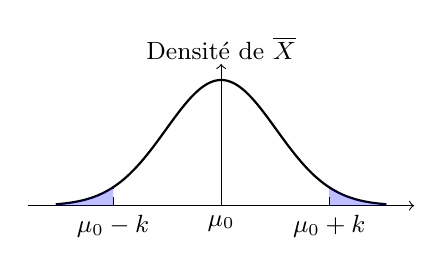
\begin{tikzpicture}[xscale=0.7, yscale=4]

\def\moy{0}
\def\sigma{1}
\def\a{1.96}

\draw[->] (-3.5,0) -- (3.5,0);
\draw[->] (0,0) -- (0,0.45);

\draw[thick, smooth, domain=-3:3, samples=200]
  plot (\x, {1/(\sigma*sqrt(2*pi)) * exp(-((\x-\moy)^2)/(2*\sigma^2))});

\path[fill=blue, fill opacity=0.25]
  plot[domain=\a:3, samples=200]
    (\x, {1/(\sigma*sqrt(2*pi)) * exp(-((\x-\moy)^2)/(2*\sigma^2))})
  -- (3,0) -- (\a,0) -- cycle;

  \path[fill=blue, fill opacity=0.25]
  plot[domain=-3:-\a, samples=200]
    (\x, {1/(\sigma*sqrt(2*pi)) * exp(-((\x-\moy)^2)/(2*\sigma^2))})
  -- (-\a,0) -- (-3,0) -- cycle;

\draw[dashed] (\a,0) --
  (\a,{1/(\sigma*sqrt(2*pi)) * exp(-((\a-\moy)^2)/(2*\sigma^2))});

\draw[dashed] (-\a,0) --
  (-\a,{1/(\sigma*sqrt(2*pi)) * exp(-((-\a-\moy)^2)/(2*\sigma^2))});
  
\node[below] at (\a,0) {\small $\mu_0+k$};
\node[below] at (-\a,0) {\small $\mu_0-k$};
\node at (0,0.5) {\small Densité de $\overline X$};
\node[below] at (0,0) {\small $\mu_0$};

\end{tikzpicture}
\end{minipage}
\hfill
\begin{minipage}{0.48\textwidth}
\centering
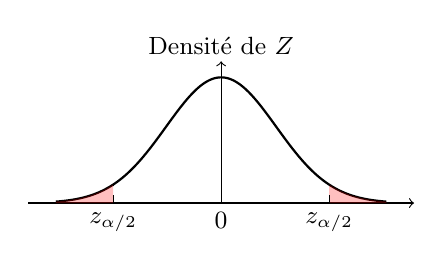
\begin{tikzpicture}[xscale=0.7, yscale=4]

\def\moy{0}
\def\sigma{1}
\def\a{1.96}

\draw[->] (-3.5,0) -- (3.5,0);
\draw[->] (0,0) -- (0,0.45);

\draw[thick, smooth, domain=-3:3, samples=200]
  plot (\x, {1/(\sigma*sqrt(2*pi)) * exp(-((\x-\moy)^2)/(2*\sigma^2))});

\path[fill=red, fill opacity=0.25]
  plot[domain=\a:3, samples=200]
    (\x, {1/(\sigma*sqrt(2*pi)) * exp(-((\x-\moy)^2)/(2*\sigma^2))})
  -- (3,0) -- (\a,0) -- cycle;
  
  \path[fill=red, fill opacity=0.25]
  plot[domain=-3:-\a, samples=200]
    (\x, {1/(\sigma*sqrt(2*pi)) * exp(-((\x-\moy)^2)/(2*\sigma^2))})
  -- (-\a,0) -- (-3,0) -- cycle;
  
\draw[dashed] (\a,0) --
  (\a,{1/(\sigma*sqrt(2*pi)) * exp(-((\a-\moy)^2)/(2*\sigma^2))});

\draw[dashed] (-\a,0) --
  (-\a,{1/(\sigma*sqrt(2*pi)) * exp(-((-\a-\moy)^2)/(2*\sigma^2))});

  
\node[below] at (\a,0) {\small $z_{\alpha/2}$};
\node[below] at (-\a,0) {\small $z_{\alpha/2}$};

\node at (0,0.5) {\small Densité de $Z$};
\node[below] at (0,0) {\small $0$};


\end{tikzpicture}
\end{minipage}
    
\end{frame}

\begin{frame}[t]{Exemple 3}

{\small
Une compagnie affirme que le remboursement d'imp\^ot moyen aux étudiants qui ont utilisé
son service est d'au moins $1100 \,\$$. \\
Un échantillon aléatoire de 20 étudiants ayant utilisé le service ont obtenu un  remboursement moyen de $1060 \,\$$. \\
En supposant une distribution normale d'écart-type $100 \,\$$ pour le remboursement d'un étudiant, peut-on conclure que la compagnie fait de la fausse publicité, au seuil $\alpha = 0,05$ ?}\\

\bigskip

{\bf 1. Hypothèses:}
\bigskip

{\bf 2. Règle de décision:}

\end{frame}

\begin{frame}[t]{Exemple 2 (suite)}

{\bf 3. Calcul de la statistique observée:}

\vfill
{\bf 4. Décision:}

L'hypothèse nulle...

\bigskip
{\bf 5. Conclusion:} (dans les termes de l'étude)

Au seuil de 5\%, le remboursement moyen ...
\bigskip
\end{frame}

\subsection{Seuil observé (valeur P)}

\begin{comment}
Une règle  du pouce est la suivante:
\begin{itemize}
\item si $\alpha^*\ge0.10$: aucune preuve contre $H_0$ (test non significatif);
\item si  $\alpha^*\in\;]0.05,0.10]$: preuve faible contre $H_0$ ;
\item si $\alpha^*\in\;]0.01,0.05]$: preuve forte contre $H_0$ ;
\item si $\alpha^*<0.01$: preuve très forte contre $H_0$ (test très significatif).
\end{itemize}
\end{comment}

\begin{frame}[t]{}

\centerline{\LARGE\bf \alert{QUIZ !}}
\medskip
Vous faites un test sur 20 observations  pour confronter les hypothèses $H_0: \mu=5$ et $H_1: \mu<5$.\\ Vous obtenez un seuil observé (valeur P) de 0,09.

Vrai, faux ou manque d'information?
\begin{enumerate}\itemsep2mm
\item La moyenne échantillonnale est inférieure à 5.
\item Vous rejetez $H_0$ au seuil de 5\%.
\item Vous rejetez $H_0$ au seuil de 10\%.
\item Vous rejetez $H_0: \mu=4$ contre $H_1: \mu<4$ au seuil de 5\%.
\item Vous rejetez $H_0: \mu=6$ contre $H_1: \mu<6$ au seuil de 5\%.
\item Vous refaites l'expérience avec 40 observations. Vous obtenez la même moyenne échantillonnale. Votre seuil observé est alors plus élevé que 0,09 pour le test $H_0: \mu=5$ contre $H_1: \mu<5$.
\end{enumerate}



\end{frame}

\begin{frame}[t]{Formules pour le seuil observé}

 {\small
 De la définition du seuil observé $\alpha^*$, on peut facilement déduire
les formules générales suivantes (pour le cas 1: loi normale, $\sigma^2$ connue):

 \begin{itemize}\itemsep4mm
 \item Pour $H_0 : \mu = \mu_0 \mbox{ vs } H_1 : \mu \neq \mu_0$:\\
 $\alpha^*=P(|Z|>|z_{0}|)=2\,P(Z>|z_{o}|)$.
 \item Pour $H_0 : \mu = \mu_0 \mbox{ vs } H_1 : \mu > \mu_0$:\\
 $\alpha^*=P(Z>z_{0})$.
 \item Pour $H_0 : \mu = \mu_0 \mbox{ vs } H_1 : \mu < \mu_0$:\\
 $\alpha^*=P(Z<z_{0})$.
 \end{itemize}
 }
\end{frame}

\begin{frame}[t]{Exemple 2 (suite)}
Quel est le seuil observé du test réalisé sur la moyenne des remboursements d'impôts?
{\ }
\end{frame}



\subsection{Puissance et taille d'échantillon}

\begin{frame}[t]{Calcul de puissance}

\begin{itemize}\itemsep7mm
\item Rappel: $$\text{Puissance du test}=P(\text{ rejeter } H_0\,|\,H_1 \text{  est vraie}).$$
\item En général, $H_1$ ne spécifie pas une valeur unique de $\mu$, mais un intervalle de valeurs.
\item On calcule la puissance pour une valeur plausible ou arbitraire de $\mu$ sous $H_1$, que nous noterons $\mu_1$.
\end{itemize}
\end{frame}

\begin{frame}[t]{Exemple 4}
On pige un échantillon $X_1, \ldots, X_{16}$  d'une loi $N(\mu, 64)$ pour tester, au seuil $\alpha = 0,10$:

 $$\begin{array}{ll}
 H_0 : &\mu = 10\\ H_1 : &\mu > 10
 \end{array}$$

 Quelle est la puissance du test si en vérité $\mu = 11$?
\end{frame}

\begin{frame}[t]{Exemple 4 (suite)}

{\ }

\end{frame}

\begin{frame}[t]{Déterminants de la puissance}

{\small
Trois facteurs importants influencent la puissance d'un test:}

\begin{enumerate}
\item[1.] \alert{la différence entre $\mu_0$ et $\mu_1$}:
plus $\mu_1$ s'éloigne de $\mu_0$, plus la puissance augmente.
\begin{center}
    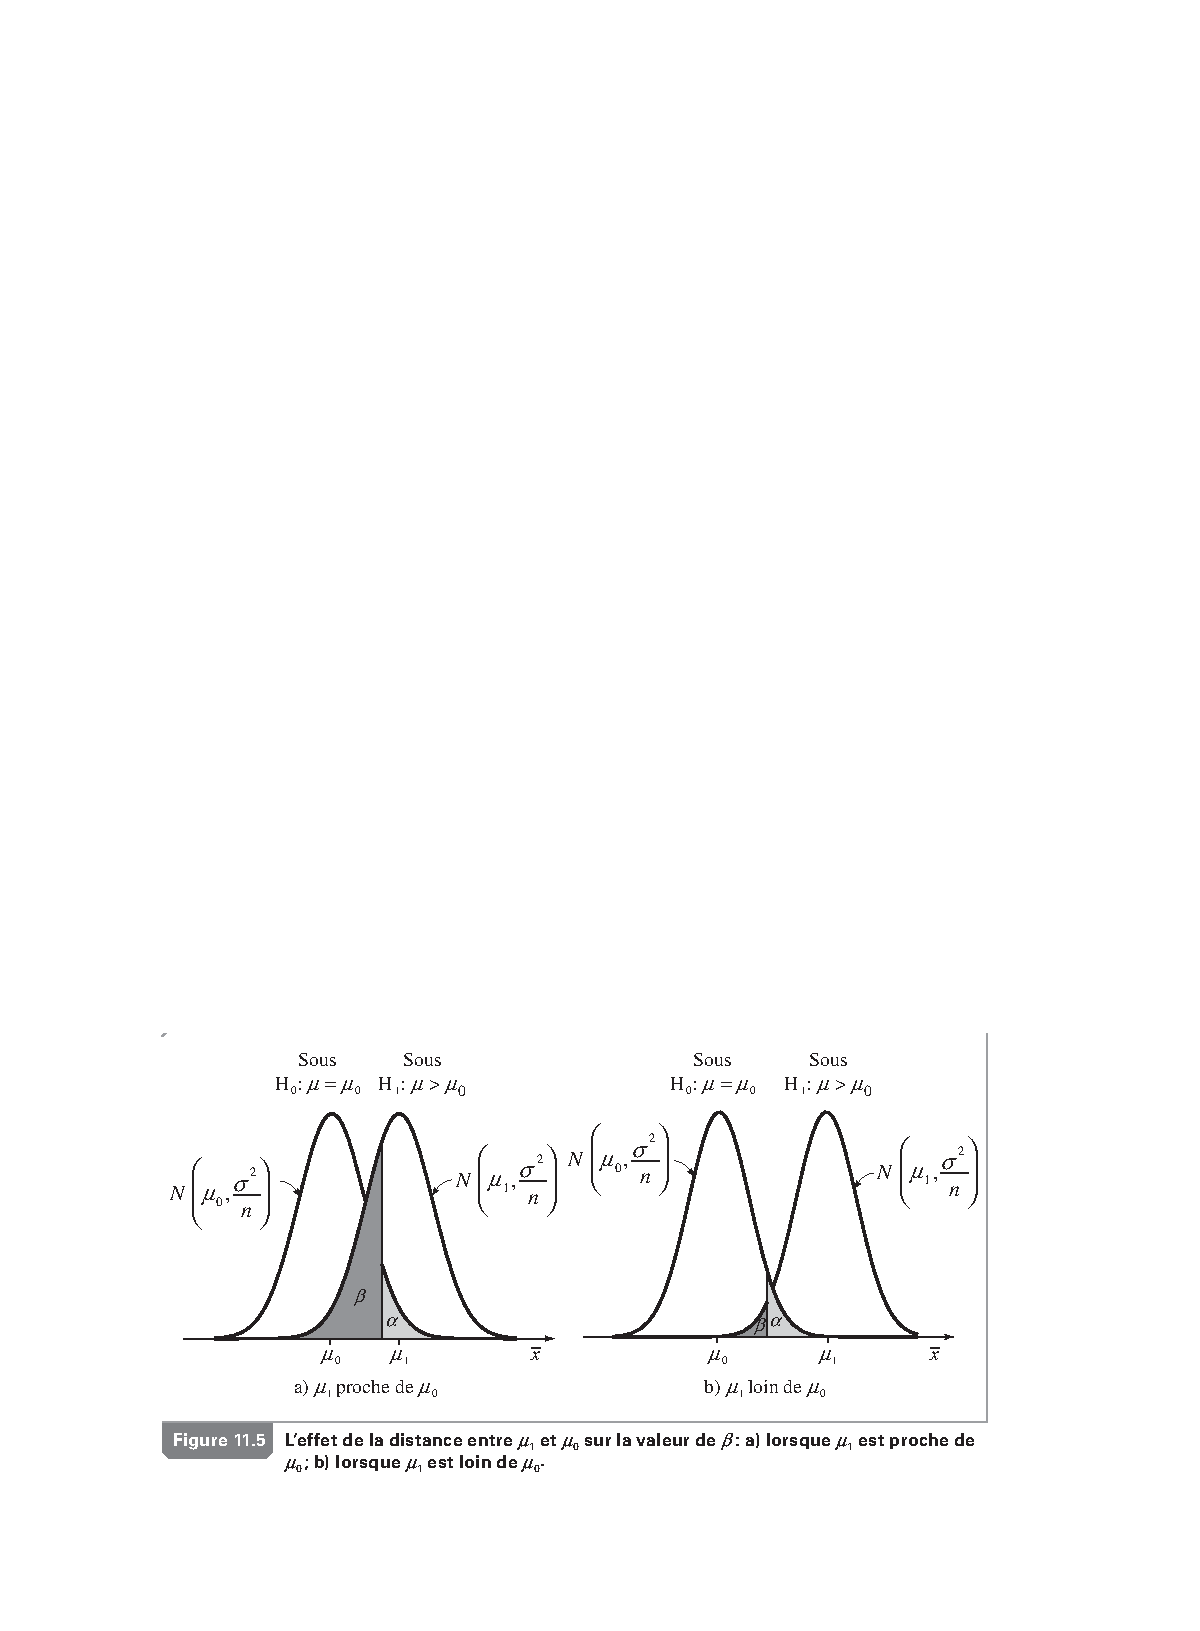
\includegraphics[scale = 0.65]{puiss1.pdf}

\end{center}

\end{enumerate}
\end{frame}

\begin{frame}[t]{Déterminants de la puissance}

\begin{enumerate}
\item[2.] \alert{le seuil du test}:
plus $\alpha$ augmente, plus la puissance augmente;

\begin{center}
    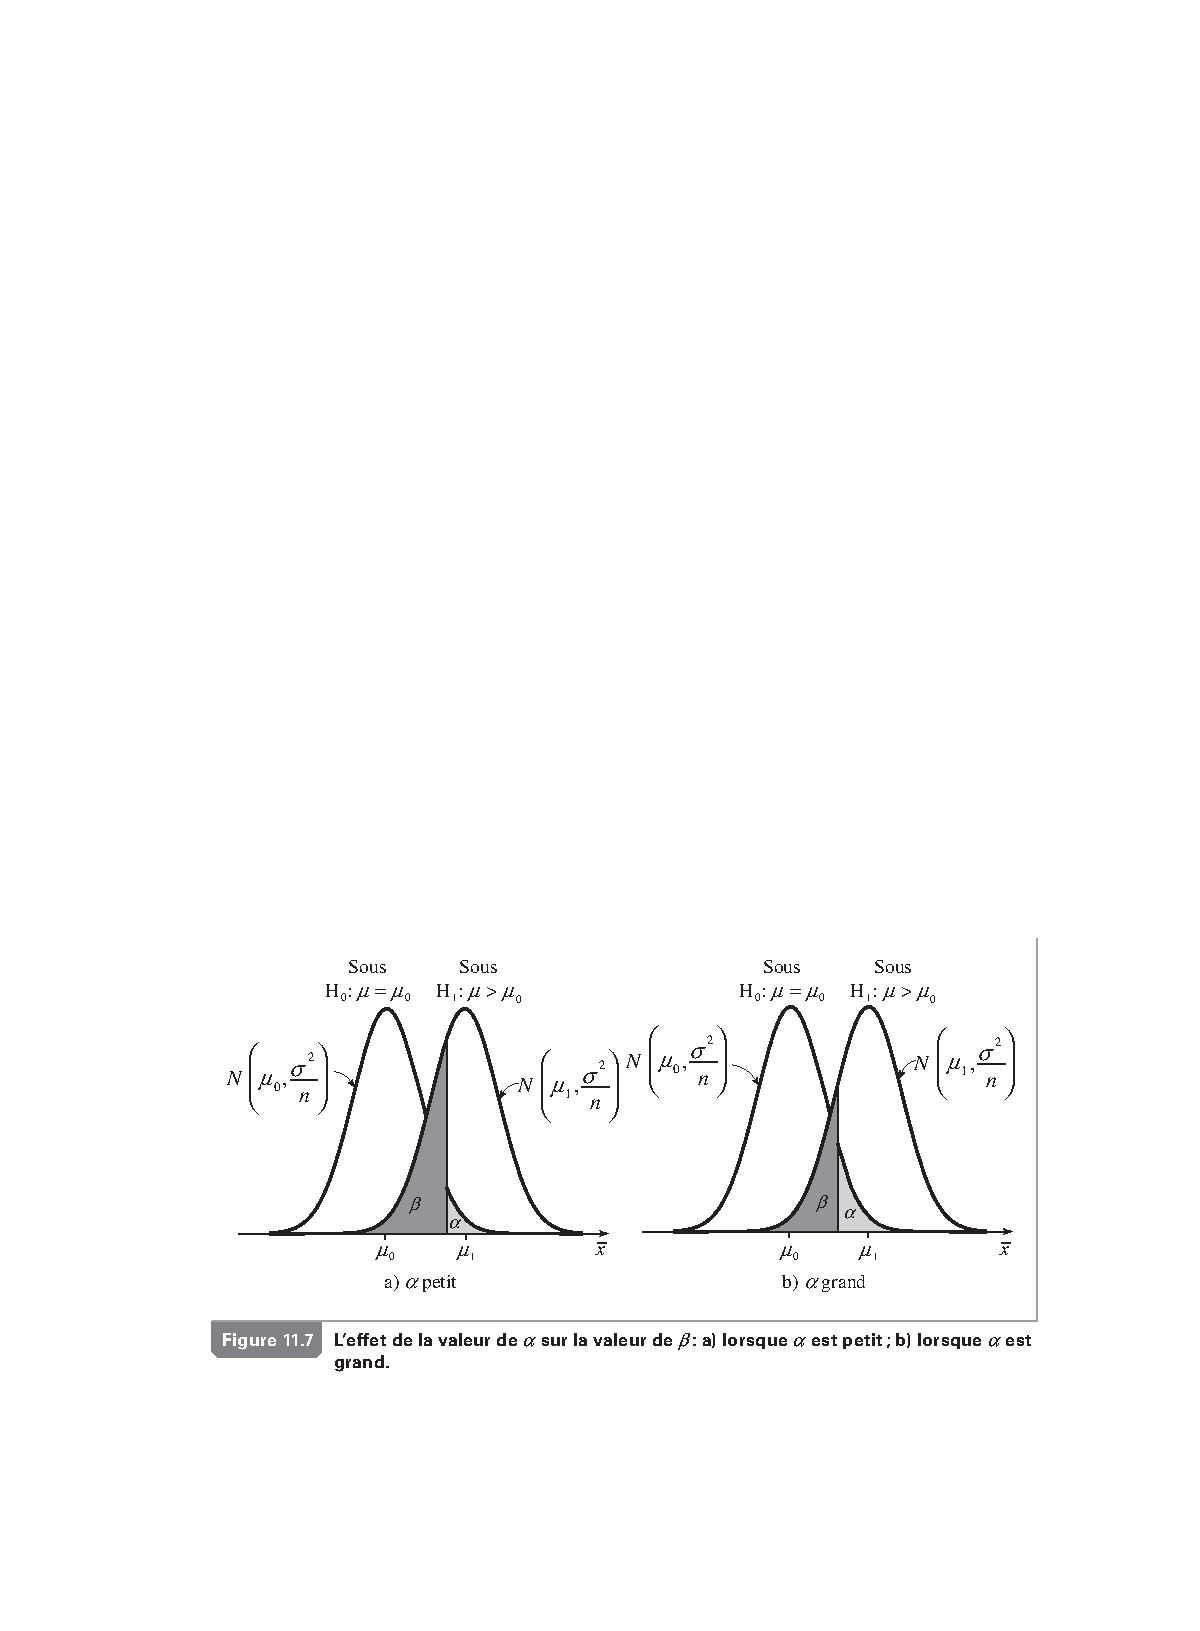
\includegraphics[scale = 0.65]{puiss3.pdf}

\end{center}
\end{enumerate}
\end{frame}


\begin{frame}[t]{Déterminants de la puissance}


\begin{enumerate}
\item[3.] \alert{la taille d'échantillon}: plus $n$ augmente, plus la puissance augmente.

\begin{center}
    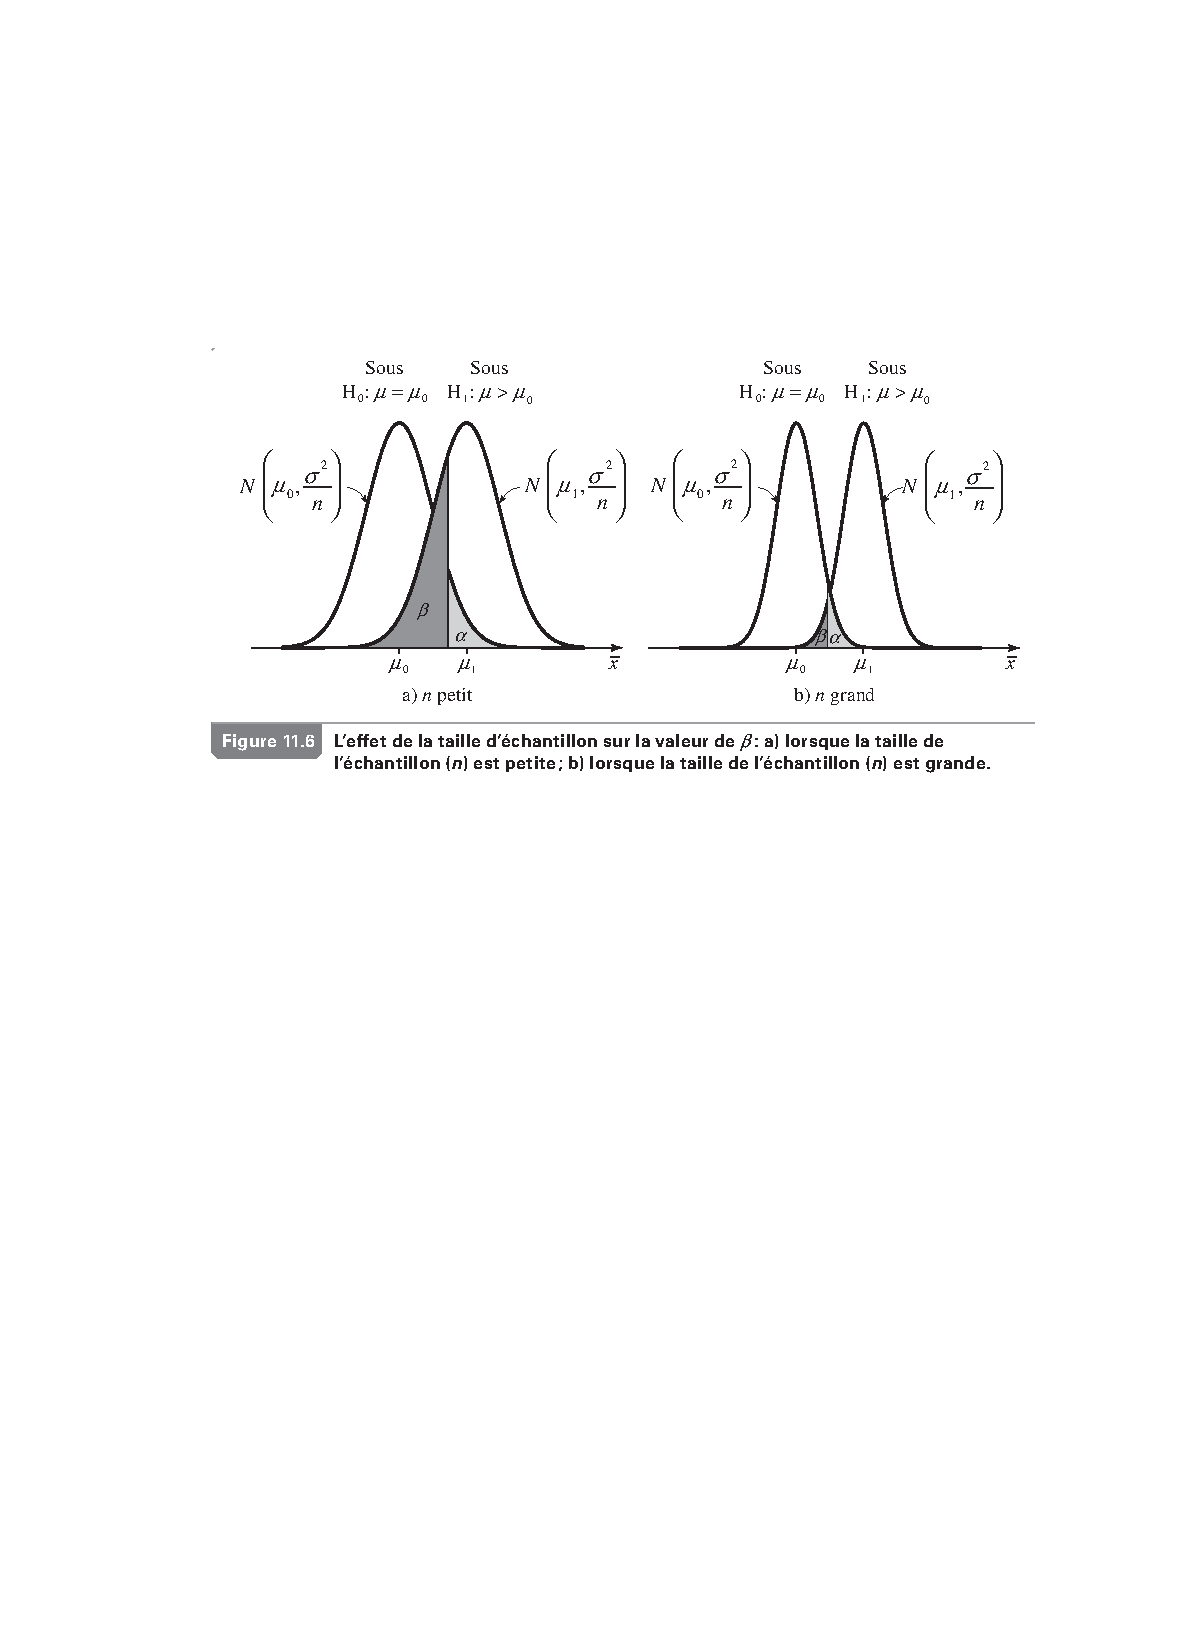
\includegraphics[scale = 0.65]{puiss2.pdf}

\end{center}

\end{enumerate}
\end{frame}
\begin{frame}[t]{Déterminants de la puissance}

\begin{enumerate}\itemsep5mm
\item Le statisticien n'a aucun contr\^ole sur $\mu$, la vraie valeur de la moyenne. Il peut demander au chercheur la plus petite différence qu'il considère importante.

\item On peut augmenter $\alpha$ pour augmenter la puissance, mais on augmente les chances de faire une erreur de type I.

\item En pratique, \alert{la seule option est souvent d'augmenter la puissance en choisissant $n$ suffisamment grand}.
\end{enumerate}
\end{frame}

\begin{frame}[t]{Exemple 4 (suite)}

On reconsidère notre échantillonnage dans une population  $N(\mu, 64)$ pour tester (avec $\alpha = 0,10$)

 $$\begin{array}{ll}
 H_0 : &\mu = 10\\ H_1 : &\mu > 10
 \end{array}$$

Quelle est la taille d'échantillon nécessaire pour que la puissance soit de 80\% si $\mu = 11$?

\end{frame}



%%%%%%%%%%%%%%%%%%%%%%%%%%%%%%%%%%%%%%%%%%%%%%%%%%%%%%%%%%%%%%%%%%%%%%%%%%%%%%%%%%%%%
\section[2)Test $\mu$ ($\sigma^2$ inconnue)]{Cas 2: Tests d'hypothèses sur la moyenne d'une distribution normale de variance inconnue}
\subsection*{ }

%\subsection{Statistique de test}

\begin{frame}[t]{Cas 2: Tests sur $\mu$,  loi normale, $\sigma^2$ inconnue}

Comment faire un test sur $\mu$ si la variance est inconnue?

\medskip
Le test basé sur $Z_0$ est inapproprié puisque l'erreur de type I qui serait commise
serait  supérieure à $\alpha$.

\medskip

Si la variance est inconnue, on utilise la statistique
$$
T_0 = \frac{\overline{X}-\mu_0}{S/\sqrt{n}}.
$$
Sous $H_0$, on sait que $T_0\sim t_{n-1}$.

\end{frame}

\begin{frame}[t]{Règles de décision}

{\small
Au seuil $\alpha$, on rejette $H_0:\mu=\mu_0$ ...
\begin{itemize}
\item \underline{Test bilatéral ($H_1 : \mu \ne \mu_0$)}:

    \begin{enumerate}[$\circ$]\itemsep2mm
    \item on rejette $H_0$ si $|t_0| > t_{\alpha/2, n-1}$
    \item $\alpha^*=P(|t_{n-1}|>|t_0|)=2\,P(t_{n-1}>|t_0|)$
    \end{enumerate}

\item \underline{Test unilatéral à droite ($H_1 : \mu > \mu_0$)}:

    \begin{enumerate}[$\circ$]\itemsep2mm
    \item on rejette $H_0 : \mu = \mu_0$  si $t_0 > t_{\alpha, n-1}$
    \item $\alpha^*=P(t_{n-1}>t_0)$
    \end{enumerate}

\item \underline{Test unilatéral à gauche ($H_1 : \mu < \mu_0$)}:

    \begin{enumerate}[$\circ$]\itemsep2mm
    \item on rejette $H_0 : \mu = \mu_0$ si $t_0 < -t_{\alpha, n-1}$.
    \item $\alpha^*=P(t_{n-1}<t_0)$
    \end{enumerate}
\end{itemize}
}
\end{frame}

%\subsection{Seuil observé}

\begin{frame}[t]{Seuils observés et puissance}

\underline{Seuils observés}:

Dans tous les cas, on peut énoncer la règle suivante:

\centerline{\alert{On rejette $H_0$ si $\alpha^*<\alpha$.}}

C'est le calcul de la valeur-P ($\alpha^*$) qui change selon le test.

\bigskip
\uncover<2->{
\underline{Puissance}:

Les calculs de puissance pour le cas 2 font appel à une loi $t$ {\it décentrée} et ne seront donc \alert{pas couverts dans ce cours}.}
\end{frame}

\begin{frame}[t]{Exemple 5}

Une fabrique achète régulièrement des transistors à un fournisseur. Les données passées montrent que le coefficient d'amplification de ces transistors avait une distribution normale de moyenne 155.

\medskip

Lors d'un nouveau contrôle sur 20 transistors, on observe un coefficient d'amplification moyen de 152 et un écart-type de 10. Peut-on admettre, au seuil de 1\%, que le coefficient  moyen a changé?


\bigskip

{\bf 1. Hypothèses:}
\bigskip

{\bf 2. Règle de décision:}

\end{frame}

\begin{frame}[t]{Exemple 5 (suite)}

{\bf 3. Calcul de la statistique observée:}

\vfill
{\bf 4. Décision:}

L'hypothèse nulle...

\bigskip
{\bf 5. Conclusion:} (dans les termes de l'étude)

Au seuil de 1\%, le coefficient d'amplification moyen ...
\bigskip

\end{frame}


%%%%%%%%%%%%%%%%%%%%%%%%%%%%%%%%%%%%%%%%%%%%%%%%%%%%%%%%%%%%%%%%%%%%%%%%%%%%%%%%%%%%%
\section[3)Test $\mu$ (loi inconnue)]{Cas 3: Tests d'hypothèses sur la moyenne d'une distribution normale de distribution inconnue ($n$ grand)}
\subsection*{ }

\begin{frame}[t]{Cas 3: Tests sur $\mu$,  loi inconnue, $n$ grand}

Si la loi théorique des observations en cause est inconnue, comment faire un test sur la moyenne?

\vspace{5mm}

Si $n$ est grand (au moins 30), le test présenté au cas 1 peut être utilisé en rempla\c{c}ant $\sigma$ par l'écart-type échantillonnal $S$ dans la définition de $Z_0$.

\vspace{5mm}

Les probabilités d'erreur de type I et II ($\alpha$ et $\beta$) seront alors approximatives (car la loi normale est un modèle approximatif pour $\overline X$ lorsque $n$ est grand).

\end{frame}


%%%%%%%%%%%%%%%%%%%%%%%%%%%%%%%%%%%%%%%%%%%%%%%%%%%%%%%%%%%%%%%%%%%%%%%%%%%%%%%%%%%%%
\section[4)Test $\sigma^2$]{Cas 4: Tests d'hypothèses sur la variance d'une distribution normale}
\subsection*{ }

%\subsection{Construction du test}

\begin{frame}[t]{Cas 4: Tests sur $\sigma^2$, distribution normale}
Si on veut contr\^oler la variabilité d'un procédé,
on peut effectuer un test d'hypothèses portant sur la variance d'une distribution.

\medskip
Ces tests sont relativement simples dans le cas o\`u nous
recueillons un \alert{échantillon aléatoire $X_1,\ldots,X_n$ issu d'une population
$N(\mu,\sigma^2)$}.
\end{frame}

\begin{frame}[t]{Test bilatéral}

%{\small
On suppose $X_1, \ldots, X_n$ un échantillon aléatoire d'une distribution $N(\mu, \sigma^2)$
pour laquelle on veut tester $$\alert{H_0 : \sigma^2 = \sigma_0^2} \mbox{ contre } \alert{H_1 : \sigma^2 \ne \sigma_0^2}.$$
On voudra rejeter $H_0$ lorsque $S^2$ sera éloignée de $\sigma^2_0$, donc pour des valeurs éloignées de $n-1$ pour la statistique
$$U_0 = \frac{(n-1)S^2}{\sigma_0^2}. $$

\uncover<2->{
Si $H_0$ est vraie, alors $U_0\sim\chi^2_{n-1}$.\\
Test de seuil $\alpha$:\\
\centerline{\alert{on rejette $H_0$ si
$u_0<\chi^2_{1-\alpha/2;n-1}$ ou si $u_0>\chi^2_{\alpha/2;n-1}$}.}
}
%}
\end{frame}

\begin{frame}[t]{Tests unilatéraux}

{\small
Au seuil $\alpha$, on rejette $H_0:\sigma^2 = \sigma_0^2$ ...
\begin{itemize}

\item \underline{Test unilatéral à droite ($H_1 : \sigma^2 > \sigma_0^2$)}:

    \begin{enumerate}[$\circ$]\itemsep2mm
    \item on rejette $H_0 : \sigma^2 = \sigma_0^2$  si $u_0>\chi^2_{\alpha;n-1}$
    \item $\alpha^*=P(\chi^2_{n-1}>u_0)$
    \end{enumerate}

\item \underline{Test unilatéral à gauche ($H_1 : \sigma^2 < \sigma_0^2$)}:

    \begin{enumerate}[$\circ$]\itemsep2mm
    \item on rejette $H_0 : \sigma^2 = \sigma_0^2$ si $u_0<\chi^2_{1-\alpha;n-1}$.
    \item $\alpha^*=P(\chi^2_{n-1}<u_0)$
    \end{enumerate}
\end{itemize}
}
\end{frame}


\begin{frame}[t]{Exemple 6}

On évalue une nouvelle machine pour remplir des sacs de sucre. La compagnie est prête à tolérer une variance de 7 g$^2$. 
Un test sur 31 sacs donne une variance échantillonnale de \mbox{8,2 g$^2$.} \\La variance est-elle trop grande au seuil \mbox{$\alpha = 0,05$?}



\bigskip

{\bf 1. Hypothèses:}
\vspace{1cm}

{\bf 2. Règle de décision:}

\end{frame}

\begin{frame}[t]{Exemple 6 (suite)}

{\bf 3. Calcul de la statistique observée:}

\vfill
{\bf 4. Décision:}

L'hypothèse nulle...

\bigskip
{\bf 5. Conclusion:} (dans les termes de l'étude)

Au seuil de 5\%, la variance des poids ...
\bigskip
\end{frame}


%%%%%%%%%%%%%%%%%%%%%%%%%%%%%%%%%%%%%%%%%%%%%%%%%%%%%%%%%%%%%%%%%%%%%%%%%%%%%%%%%%%%%
\section[Lien IC]{Lien entre intervalles de confiance et tests d'hypothèses bilatéraux}
\subsection*{ }

\begin{frame}[t]{Intervalles de confiance et tests bilatéraux}
Il existe une forte relation entre les intervalles de confiance et les  tests  bilatéraux.

\bigskip
L'examen des régions critiques des tests pour
 $H_0:~\mu=\mu_0$ vs $H_1:~\mu\neq\mu_0$ montre que
 \bigskip

 \begin{tabular}{c c l}
 \alert{On rejette $H_0:~\mu=\mu_0$ }&  &
 \alert{L'intervalle de confiance pour $\mu$ }\\
 \alert{au seuil $\alpha$}& $\Leftrightarrow$ &\alert{de niveau $1-\alpha$ }\\
 &&\alert{ne
 contient pas la valeur $\mu_0$}.
 \end{tabular}

 \vspace{1.8cm}

 Idem pour $\sigma^2$.
\end{frame}

\begin{frame}[t]{ }

\centerline{\LARGE\bf \alert{QUIZ !}}
\bigskip

À la suite d'une étude, on a calculé un intervalle de confiance à 99\% pour $\mu$: $[2,26;\,3,41]$.

\bigskip
Vrai, faux, ou info insuffisante?

\begin{enumerate}\itemsep 8mm
\item Au seuil de 1\%, on rejette $H_0:\mu=3$ pour $H_1:\mu\ne3$.
\item Au seuil de 1\%, on rejette $H_0:\mu=4$ pour $H_1:\mu\ne4$.
\item Au seuil de 5\%, on rejette $H_0:\mu=3$ pour $H_1:\mu\ne3$.
\item Au seuil de 5\%, on rejette $H_0:\mu=4$ pour $H_1:\mu\ne4$.
\end{enumerate}


\end{frame}

\begin{frame}[t]{Réponses aux exemples}

{\scriptsize

\begin{enumerate}
  \item $H_0:\mu=0,10$ contre $H_1: \mu>0,10$. $\quad\alpha_1>\alpha_2; \quad\beta_1<\beta_2 \quad1-\beta_1>1-\beta_2$. ($\alpha^*=0,041$)
  \item $\alpha^*\approx 0,33~\%$, alors que $P(H_0\text{\ est vraie}\;|\;X=4)\approx13,56\%$
  \item $H_0:\mu=1100$ contre $H_1: \mu<1100$. Rejet de $H_0$ si $z_0<-1,645$. $z_0=-1,79$, donc le remboursement moyen est significativement inférieur à 1100 \$. ($\alpha^*=0,037$)
  \item $1-\beta = 0,218$, $n=291$
  \item $H_0:\mu=155$ contre $H_1: \mu\ne 155$. Rejet de $H_0$ si $|T_0|>2,861$. $T_0=-1,34$, donc le changement de moyenne n'est pas significatif au seuil de 1\%. ($\alpha^*=0,196$)
  \item  $H_0:\sigma^2=7$ contre $H_1: \sigma^2>7$. Rejet de $H_0$ si $U_0>43,77$. $U_0=35,14$, donc la variance n'est pas significativement trop grande au seuil de 5\%. ($\alpha^*=0,238$)
 \end{enumerate}
 }
\end{frame}


\end{document}